%TR 100
\begin{figure}[H]
    \caption{Curva ajustada para os dados para TR 100 anos e 1 neurônio artificial}
    \centering
    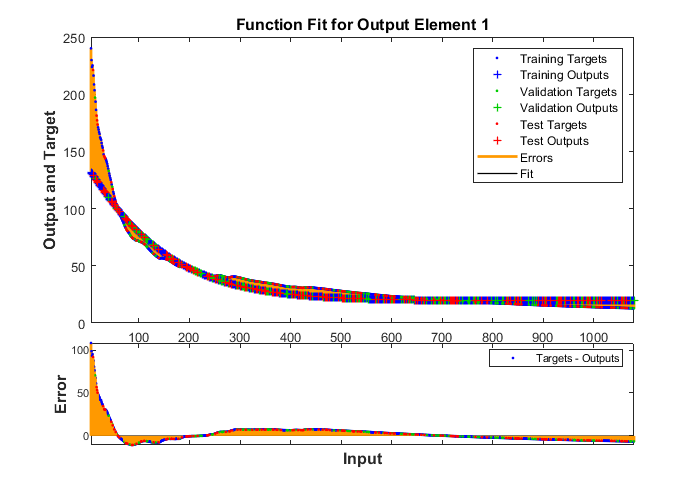
\includegraphics[width=0.74\textwidth]{Textuais/Figuras/NN/tr100-1neuronio.png}
    \fonte{Autores}
    \label{fig:tr100-1n}
\end{figure}

\begin{figure}[H]
    \caption{Curva ajustada para os dados para TR 100 anos e 2 neurônios artificiais}
    \centering
    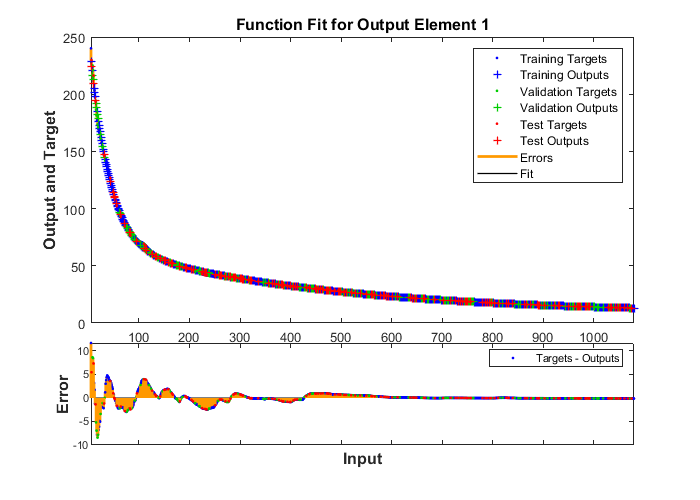
\includegraphics[width=0.74\textwidth]{Textuais/Figuras/NN/tr100-2neuronio.png}
    \fonte{Autores}
    \label{fig:tr100-2n}
\end{figure}

\begin{figure}[H]
    \caption{Curva ajustada para os dados para TR 100 anos e 5 neurônios artificiais}
    \centering
    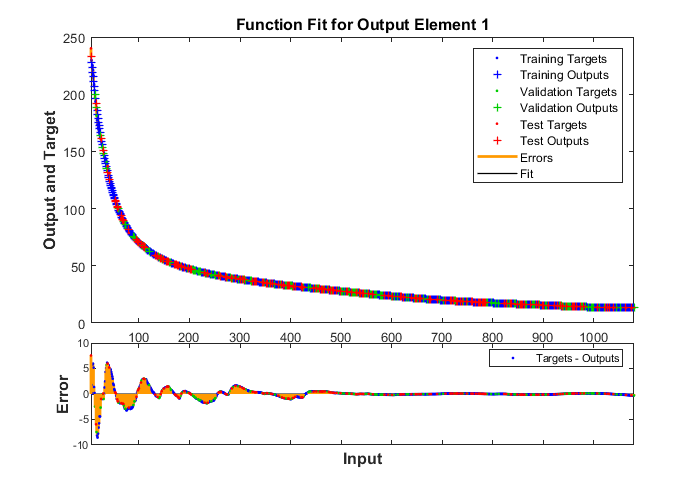
\includegraphics[width=0.74\textwidth]{Textuais/Figuras/NN/tr100-5neuronio.png}
    \fonte{Autores}
    \label{fig:tr100-5n}
\end{figure}

\begin{figure}[H]
    \caption{Curva ajustada para os dados para TR 100 anos e 10 neurônios artificiais}
    \centering
    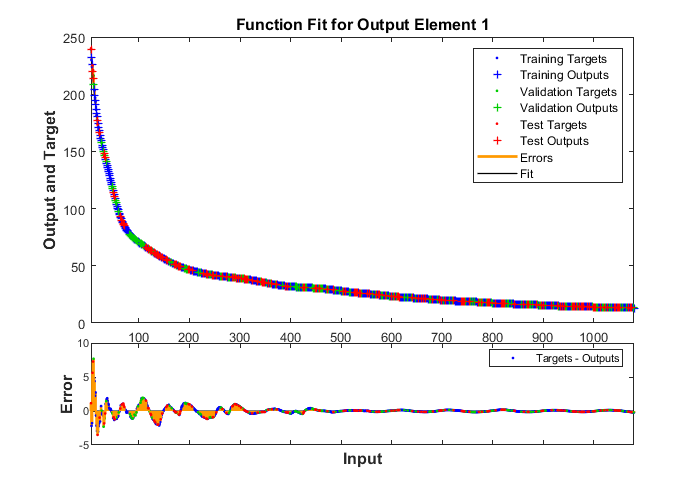
\includegraphics[width=0.74\textwidth]{Textuais/Figuras/NN/tr100-10neuronio.png}
    \fonte{Autores}
    \label{fig:tr100-10n}
\end{figure}
%FIM TR 100

\begin{figure}[H]
    \caption{Comparação entre as curvas geradas para TR100 e 10 neurônios}
    \centering
    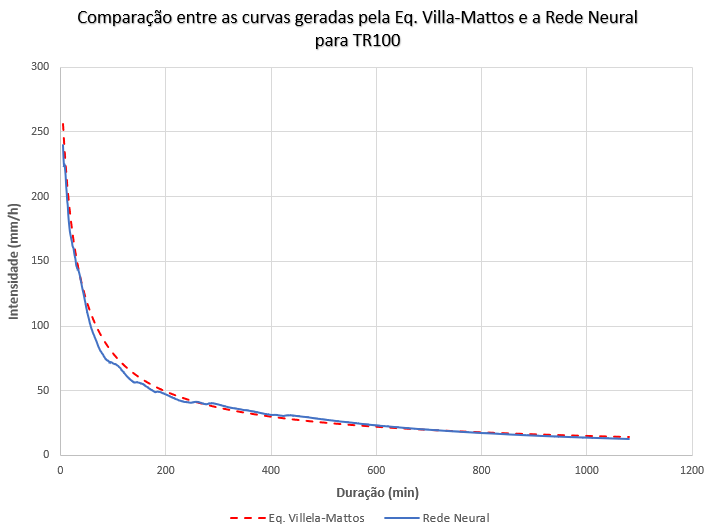
\includegraphics[width=\textwidth]{Textuais/Resultados/Comparacao/TR100.png}
    \fonte{Autores}
    \label{fig:comp-tr100}
\end{figure}